% Options for packages loaded elsewhere
\PassOptionsToPackage{unicode}{hyperref}
\PassOptionsToPackage{hyphens}{url}
%
\documentclass[
]{article}
\usepackage{amsmath,amssymb}
\usepackage{lmodern}
\usepackage{iftex}
\ifPDFTeX
  \usepackage[T1]{fontenc}
  \usepackage[utf8]{inputenc}
  \usepackage{textcomp} % provide euro and other symbols
\else % if luatex or xetex
  \usepackage{unicode-math}
  \defaultfontfeatures{Scale=MatchLowercase}
  \defaultfontfeatures[\rmfamily]{Ligatures=TeX,Scale=1}
\fi
% Use upquote if available, for straight quotes in verbatim environments
\IfFileExists{upquote.sty}{\usepackage{upquote}}{}
\IfFileExists{microtype.sty}{% use microtype if available
  \usepackage[]{microtype}
  \UseMicrotypeSet[protrusion]{basicmath} % disable protrusion for tt fonts
}{}
\makeatletter
\@ifundefined{KOMAClassName}{% if non-KOMA class
  \IfFileExists{parskip.sty}{%
    \usepackage{parskip}
  }{% else
    \setlength{\parindent}{0pt}
    \setlength{\parskip}{6pt plus 2pt minus 1pt}}
}{% if KOMA class
  \KOMAoptions{parskip=half}}
\makeatother
\usepackage{xcolor}
\usepackage[margin=1in]{geometry}
\usepackage{color}
\usepackage{fancyvrb}
\newcommand{\VerbBar}{|}
\newcommand{\VERB}{\Verb[commandchars=\\\{\}]}
\DefineVerbatimEnvironment{Highlighting}{Verbatim}{commandchars=\\\{\}}
% Add ',fontsize=\small' for more characters per line
\usepackage{framed}
\definecolor{shadecolor}{RGB}{248,248,248}
\newenvironment{Shaded}{\begin{snugshade}}{\end{snugshade}}
\newcommand{\AlertTok}[1]{\textcolor[rgb]{0.94,0.16,0.16}{#1}}
\newcommand{\AnnotationTok}[1]{\textcolor[rgb]{0.56,0.35,0.01}{\textbf{\textit{#1}}}}
\newcommand{\AttributeTok}[1]{\textcolor[rgb]{0.77,0.63,0.00}{#1}}
\newcommand{\BaseNTok}[1]{\textcolor[rgb]{0.00,0.00,0.81}{#1}}
\newcommand{\BuiltInTok}[1]{#1}
\newcommand{\CharTok}[1]{\textcolor[rgb]{0.31,0.60,0.02}{#1}}
\newcommand{\CommentTok}[1]{\textcolor[rgb]{0.56,0.35,0.01}{\textit{#1}}}
\newcommand{\CommentVarTok}[1]{\textcolor[rgb]{0.56,0.35,0.01}{\textbf{\textit{#1}}}}
\newcommand{\ConstantTok}[1]{\textcolor[rgb]{0.00,0.00,0.00}{#1}}
\newcommand{\ControlFlowTok}[1]{\textcolor[rgb]{0.13,0.29,0.53}{\textbf{#1}}}
\newcommand{\DataTypeTok}[1]{\textcolor[rgb]{0.13,0.29,0.53}{#1}}
\newcommand{\DecValTok}[1]{\textcolor[rgb]{0.00,0.00,0.81}{#1}}
\newcommand{\DocumentationTok}[1]{\textcolor[rgb]{0.56,0.35,0.01}{\textbf{\textit{#1}}}}
\newcommand{\ErrorTok}[1]{\textcolor[rgb]{0.64,0.00,0.00}{\textbf{#1}}}
\newcommand{\ExtensionTok}[1]{#1}
\newcommand{\FloatTok}[1]{\textcolor[rgb]{0.00,0.00,0.81}{#1}}
\newcommand{\FunctionTok}[1]{\textcolor[rgb]{0.00,0.00,0.00}{#1}}
\newcommand{\ImportTok}[1]{#1}
\newcommand{\InformationTok}[1]{\textcolor[rgb]{0.56,0.35,0.01}{\textbf{\textit{#1}}}}
\newcommand{\KeywordTok}[1]{\textcolor[rgb]{0.13,0.29,0.53}{\textbf{#1}}}
\newcommand{\NormalTok}[1]{#1}
\newcommand{\OperatorTok}[1]{\textcolor[rgb]{0.81,0.36,0.00}{\textbf{#1}}}
\newcommand{\OtherTok}[1]{\textcolor[rgb]{0.56,0.35,0.01}{#1}}
\newcommand{\PreprocessorTok}[1]{\textcolor[rgb]{0.56,0.35,0.01}{\textit{#1}}}
\newcommand{\RegionMarkerTok}[1]{#1}
\newcommand{\SpecialCharTok}[1]{\textcolor[rgb]{0.00,0.00,0.00}{#1}}
\newcommand{\SpecialStringTok}[1]{\textcolor[rgb]{0.31,0.60,0.02}{#1}}
\newcommand{\StringTok}[1]{\textcolor[rgb]{0.31,0.60,0.02}{#1}}
\newcommand{\VariableTok}[1]{\textcolor[rgb]{0.00,0.00,0.00}{#1}}
\newcommand{\VerbatimStringTok}[1]{\textcolor[rgb]{0.31,0.60,0.02}{#1}}
\newcommand{\WarningTok}[1]{\textcolor[rgb]{0.56,0.35,0.01}{\textbf{\textit{#1}}}}
\usepackage{graphicx}
\makeatletter
\def\maxwidth{\ifdim\Gin@nat@width>\linewidth\linewidth\else\Gin@nat@width\fi}
\def\maxheight{\ifdim\Gin@nat@height>\textheight\textheight\else\Gin@nat@height\fi}
\makeatother
% Scale images if necessary, so that they will not overflow the page
% margins by default, and it is still possible to overwrite the defaults
% using explicit options in \includegraphics[width, height, ...]{}
\setkeys{Gin}{width=\maxwidth,height=\maxheight,keepaspectratio}
% Set default figure placement to htbp
\makeatletter
\def\fps@figure{htbp}
\makeatother
\setlength{\emergencystretch}{3em} % prevent overfull lines
\providecommand{\tightlist}{%
  \setlength{\itemsep}{0pt}\setlength{\parskip}{0pt}}
\setcounter{secnumdepth}{-\maxdimen} % remove section numbering
\ifLuaTeX
  \usepackage{selnolig}  % disable illegal ligatures
\fi
\IfFileExists{bookmark.sty}{\usepackage{bookmark}}{\usepackage{hyperref}}
\IfFileExists{xurl.sty}{\usepackage{xurl}}{} % add URL line breaks if available
\urlstyle{same} % disable monospaced font for URLs
\hypersetup{
  pdftitle={R Notebook},
  hidelinks,
  pdfcreator={LaTeX via pandoc}}

\title{R Notebook}
\author{}
\date{\vspace{-2.5em}}

\begin{document}
\maketitle

\begin{Shaded}
\begin{Highlighting}[]
\FunctionTok{library}\NormalTok{(tidyverse)}
\end{Highlighting}
\end{Shaded}

\begin{verbatim}
## -- Attaching core tidyverse packages ------------------------ tidyverse 2.0.0 --
## v dplyr     1.1.0     v readr     2.1.4
## v forcats   1.0.0     v stringr   1.5.0
## v ggplot2   3.4.1     v tibble    3.1.8
## v lubridate 1.9.2     v tidyr     1.3.0
## v purrr     1.0.1     
## -- Conflicts ------------------------------------------ tidyverse_conflicts() --
## x dplyr::filter() masks stats::filter()
## x dplyr::lag()    masks stats::lag()
## i Use the ]8;;http://conflicted.r-lib.org/conflicted package]8;; to force all conflicts to become errors
\end{verbatim}

\begin{Shaded}
\begin{Highlighting}[]
\FunctionTok{library}\NormalTok{(dplyr)}
\end{Highlighting}
\end{Shaded}

\hypertarget{project-1}{%
\section{Project 1}\label{project-1}}

Loading the file

\begin{Shaded}
\begin{Highlighting}[]
\NormalTok{female }\OtherTok{\textless{}{-}} \FunctionTok{read.csv}\NormalTok{(}\StringTok{"female.csv"}\NormalTok{)}
\end{Highlighting}
\end{Shaded}

\begin{Shaded}
\begin{Highlighting}[]
\CommentTok{\# Determine whether the female dataset is a data frame}
\FunctionTok{is.data.frame}\NormalTok{(female)}
\end{Highlighting}
\end{Shaded}

\begin{verbatim}
## [1] TRUE
\end{verbatim}

\begin{Shaded}
\begin{Highlighting}[]
\CommentTok{\# printing the first few rows of the data frame}
\FunctionTok{head}\NormalTok{(female)}
\end{Highlighting}
\end{Shaded}

\begin{verbatim}
##                                                                                                               Series.Name
## 1 Account ownership at a financial institution or with a mobile-money-service provider, female (% of population ages 15+)
## 2 Account ownership at a financial institution or with a mobile-money-service provider, female (% of population ages 15+)
## 3 Account ownership at a financial institution or with a mobile-money-service provider, female (% of population ages 15+)
## 4 Account ownership at a financial institution or with a mobile-money-service provider, female (% of population ages 15+)
## 5 Account ownership at a financial institution or with a mobile-money-service provider, female (% of population ages 15+)
## 6 Account ownership at a financial institution or with a mobile-money-service provider, female (% of population ages 15+)
##         Series.Code   Country.Name Country.Code X1990..YR1990. X2000..YR2000.
## 1 FX.OWN.TOTL.FE.ZS    Afghanistan          AFG             ..             ..
## 2 FX.OWN.TOTL.FE.ZS        Albania          ALB             ..             ..
## 3 FX.OWN.TOTL.FE.ZS        Algeria          DZA             ..             ..
## 4 FX.OWN.TOTL.FE.ZS American Samoa          ASM             ..             ..
## 5 FX.OWN.TOTL.FE.ZS        Andorra          AND             ..             ..
## 6 FX.OWN.TOTL.FE.ZS         Angola          AGO             ..             ..
##   X2012..YR2012. X2013..YR2013. X2014..YR2014. X2015..YR2015. X2016..YR2016.
## 1             ..             ..           3.81             ..             ..
## 2             ..             ..          33.59             ..             ..
## 3             ..             ..          40.07             ..             ..
## 4             ..             ..             ..             ..             ..
## 5             ..             ..             ..             ..             ..
## 6             ..             ..          22.33             ..             ..
##   X2017..YR2017. X2018..YR2018. X2019..YR2019. X2020..YR2020. X2021..YR2021.
## 1           7.16             ..             ..             ..            4.7
## 2           38.1             ..             ..             ..          45.69
## 3          29.27             ..             ..             ..          31.19
## 4             ..             ..             ..             ..             ..
## 5             ..             ..             ..             ..             ..
## 6             ..             ..             ..             ..             ..
\end{verbatim}

\begin{Shaded}
\begin{Highlighting}[]
\CommentTok{\# selecting rows we want to use in our analysis}
\NormalTok{female }\OtherTok{\textless{}{-}}\NormalTok{ female }\SpecialCharTok{\%\textgreater{}\%}
\FunctionTok{filter}\NormalTok{(Country.Name }\SpecialCharTok{==} \StringTok{"Brazil"} \SpecialCharTok{|}\NormalTok{ Country.Name }\SpecialCharTok{==} \StringTok{"India"} \SpecialCharTok{|}\NormalTok{ Country.Name }\SpecialCharTok{==} \StringTok{"United States"}\NormalTok{)}
\end{Highlighting}
\end{Shaded}

\begin{Shaded}
\begin{Highlighting}[]
\CommentTok{\# we remove the null and unnecessary columns and then rename the columns}
\NormalTok{female }\OtherTok{\textless{}{-}}\NormalTok{ female[ }\SpecialCharTok{{-}}\FunctionTok{c}\NormalTok{(}\DecValTok{1}\NormalTok{,}\DecValTok{2}\NormalTok{,}\DecValTok{4}\NormalTok{,}\DecValTok{5}\SpecialCharTok{:}\DecValTok{8}\NormalTok{,}\DecValTok{10}\SpecialCharTok{:}\DecValTok{11}\NormalTok{,}\DecValTok{13}\SpecialCharTok{:}\DecValTok{15}\NormalTok{)] }\SpecialCharTok{\%\textgreater{}\%}
  \FunctionTok{rename}\NormalTok{(}\StringTok{"2014"} \OtherTok{=} \DecValTok{2}\NormalTok{, }\StringTok{"2017"} \OtherTok{=} \DecValTok{3}\NormalTok{, }\StringTok{"2021"} \OtherTok{=} \DecValTok{4}\NormalTok{)}

\FunctionTok{head}\NormalTok{(female)}
\end{Highlighting}
\end{Shaded}

\begin{verbatim}
##    Country.Name  2014  2017  2021
## 1        Brazil 64.77 67.51 80.87
## 2         India 43.13 76.64 77.55
## 3 United States  94.8 92.69 96.79
\end{verbatim}

\begin{Shaded}
\begin{Highlighting}[]
\CommentTok{\# we flip the rows and columns of the dataframe (transpose) and remove the first column}
\NormalTok{transpose\_f }\OtherTok{\textless{}{-}} \FunctionTok{data.frame}\NormalTok{(}\FunctionTok{t}\NormalTok{(female[}\SpecialCharTok{{-}}\DecValTok{1}\NormalTok{]))}
\CommentTok{\# Assign new columns from  the first column of the original df}
\FunctionTok{colnames}\NormalTok{(transpose\_f) }\OtherTok{\textless{}{-}}\NormalTok{ female[, }\DecValTok{1}\NormalTok{]}

\FunctionTok{head}\NormalTok{(transpose\_f)}
\end{Highlighting}
\end{Shaded}

\begin{verbatim}
##      Brazil India United States
## 2014  64.77 43.13          94.8
## 2017  67.51 76.64         92.69
## 2021  80.87 77.55         96.79
\end{verbatim}

\begin{Shaded}
\begin{Highlighting}[]
\CommentTok{\#}
\CommentTok{\# return a class of each column using the supply function that takes a list, vector, and return a vector of the results.}
\FunctionTok{print}\NormalTok{(}\FunctionTok{sapply}\NormalTok{(transpose\_f, class))}
\end{Highlighting}
\end{Shaded}

\begin{verbatim}
##        Brazil         India United States 
##   "character"   "character"   "character"
\end{verbatim}

\begin{Shaded}
\begin{Highlighting}[]
\CommentTok{\# turn the entries to numeric}

\NormalTok{transpose\_f}\SpecialCharTok{$}\NormalTok{Brazil }\OtherTok{=} \FunctionTok{as.numeric}\NormalTok{(}\FunctionTok{as.character}\NormalTok{(transpose\_f}\SpecialCharTok{$}\NormalTok{Brazil))}
\NormalTok{transpose\_f}\SpecialCharTok{$}\NormalTok{India }\OtherTok{=} \FunctionTok{as.numeric}\NormalTok{(}\FunctionTok{as.character}\NormalTok{(transpose\_f}\SpecialCharTok{$}\NormalTok{India))}
\NormalTok{transpose\_f}\SpecialCharTok{$}\StringTok{"United States"} \OtherTok{=} \FunctionTok{as.numeric}\NormalTok{(}\FunctionTok{as.character}\NormalTok{((transpose\_f}\SpecialCharTok{$}\StringTok{"United States"}\NormalTok{)))}

\FunctionTok{head}\NormalTok{(transpose\_f)}
\end{Highlighting}
\end{Shaded}

\begin{verbatim}
##      Brazil India United States
## 2014  64.77 43.13         94.80
## 2017  67.51 76.64         92.69
## 2021  80.87 77.55         96.79
\end{verbatim}

\begin{Shaded}
\begin{Highlighting}[]
\CommentTok{\# summarize each column with mean}
\FunctionTok{summarise\_each}\NormalTok{(transpose\_f, }\FunctionTok{list}\NormalTok{(mean))}
\end{Highlighting}
\end{Shaded}

\begin{verbatim}
## Warning: `summarise_each_()` was deprecated in dplyr 0.7.0.
## i Please use `across()` instead.
## i The deprecated feature was likely used in the dplyr package.
##   Please report the issue at <]8;;https://github.com/tidyverse/dplyr/issueshttps://github.com/tidyverse/dplyr/issues]8;;>.
\end{verbatim}

\begin{verbatim}
##   Brazil    India United States
## 1  71.05 65.77333         94.76
\end{verbatim}

\begin{Shaded}
\begin{Highlighting}[]
\CommentTok{\# Plot the change in ownership percentage overtime for the data from India }
\NormalTok{year }\OtherTok{\textless{}{-}} \FunctionTok{c}\NormalTok{(}\DecValTok{2014}\NormalTok{, }\DecValTok{2017}\NormalTok{, }\DecValTok{2021}\NormalTok{)}

\FunctionTok{ggplot}\NormalTok{(}\AttributeTok{data=}\NormalTok{transpose\_f, }\FunctionTok{aes}\NormalTok{(}\AttributeTok{x=}\NormalTok{year, }\AttributeTok{y=}\NormalTok{India, }\AttributeTok{group=}\DecValTok{1}\NormalTok{)) }\SpecialCharTok{+}
  \FunctionTok{geom\_line}\NormalTok{() }\SpecialCharTok{+}
  \FunctionTok{geom\_point}\NormalTok{()}
\end{Highlighting}
\end{Shaded}

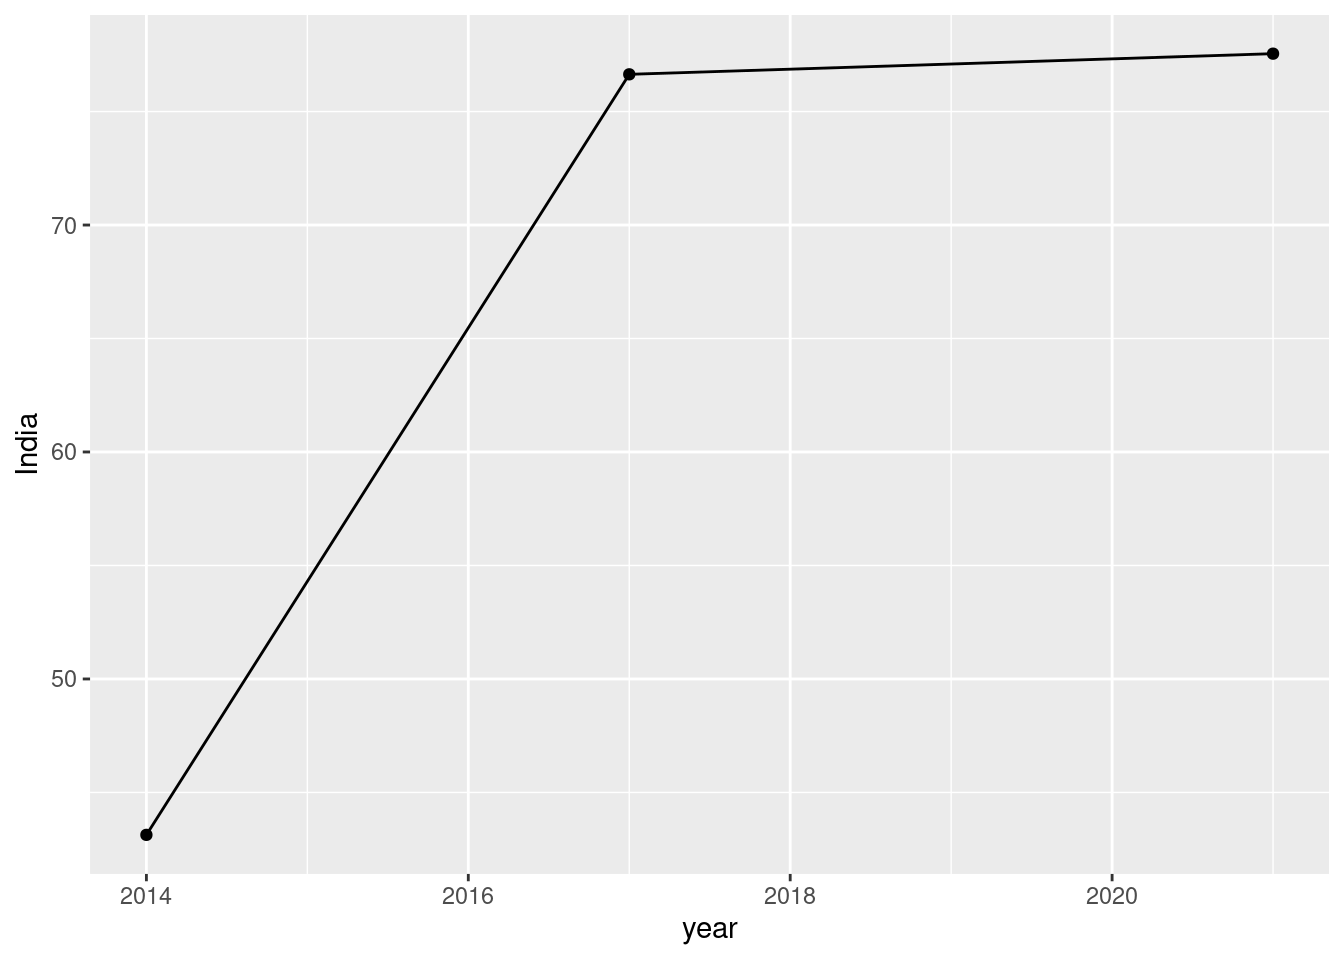
\includegraphics{myproject_files/figure-latex/unnamed-chunk-12-1.pdf}
Merging two datasets together .

\begin{Shaded}
\begin{Highlighting}[]
\NormalTok{male }\OtherTok{\textless{}{-}} \FunctionTok{read.csv}\NormalTok{(}\AttributeTok{file =} \StringTok{"male.csv"}\NormalTok{)}
\NormalTok{male }\OtherTok{\textless{}{-}}\NormalTok{ male }\SpecialCharTok{\%\textgreater{}\%}
  \FunctionTok{filter}\NormalTok{(Country.Name }\SpecialCharTok{==} \StringTok{"Brazil"} \SpecialCharTok{|}\NormalTok{ Country.Name }\SpecialCharTok{==} \StringTok{"India"} \SpecialCharTok{|}\NormalTok{ Country.Name }\SpecialCharTok{==} \StringTok{"United States"}\NormalTok{)}

\NormalTok{male }\OtherTok{\textless{}{-}}\NormalTok{ male[ }\SpecialCharTok{{-}}\FunctionTok{c}\NormalTok{(}\DecValTok{1}\NormalTok{,}\DecValTok{2}\NormalTok{,}\DecValTok{4}\NormalTok{,}\DecValTok{5}\SpecialCharTok{:}\DecValTok{8}\NormalTok{,}\DecValTok{10}\SpecialCharTok{:}\DecValTok{11}\NormalTok{,}\DecValTok{13}\SpecialCharTok{:}\DecValTok{15}\NormalTok{)] }\SpecialCharTok{\%\textgreater{}\%}
  \FunctionTok{rename}\NormalTok{(}\StringTok{"2014"} \OtherTok{=} \DecValTok{2}\NormalTok{, }\StringTok{"2017"} \OtherTok{=} \DecValTok{3}\NormalTok{, }\StringTok{"2021"} \OtherTok{=} \DecValTok{4}\NormalTok{)}

\NormalTok{transpose\_m }\OtherTok{\textless{}{-}} \FunctionTok{data.frame}\NormalTok{(}\FunctionTok{t}\NormalTok{(male[}\SpecialCharTok{{-}}\DecValTok{1}\NormalTok{]))}
\FunctionTok{colnames}\NormalTok{(transpose\_m) }\OtherTok{\textless{}{-}}\NormalTok{ male[, }\DecValTok{1}\NormalTok{]}

\NormalTok{transpose\_m}\SpecialCharTok{$}\NormalTok{Brazil }\OtherTok{=} \FunctionTok{as.numeric}\NormalTok{(}\FunctionTok{as.character}\NormalTok{(transpose\_m}\SpecialCharTok{$}\NormalTok{Brazil))}
\NormalTok{transpose\_m}\SpecialCharTok{$}\NormalTok{India }\OtherTok{=} \FunctionTok{as.numeric}\NormalTok{(}\FunctionTok{as.character}\NormalTok{(transpose\_m}\SpecialCharTok{$}\NormalTok{India))}
\NormalTok{transpose\_m}\SpecialCharTok{$}\StringTok{"United States"} \OtherTok{=} \FunctionTok{as.numeric}\NormalTok{(}\FunctionTok{as.character}\NormalTok{((transpose\_m}\SpecialCharTok{$}\StringTok{"United States"}\NormalTok{)))}


\FunctionTok{head}\NormalTok{(transpose\_m)}
\end{Highlighting}
\end{Shaded}

\begin{verbatim}
##      Brazil India United States
## 2014  71.69 62.76         92.36
## 2017  72.85 83.01         93.57
## 2021  87.05 77.51         93.09
\end{verbatim}

\begin{Shaded}
\begin{Highlighting}[]
\NormalTok{transpose\_m }\OtherTok{\textless{}{-}} \FunctionTok{rename}\NormalTok{(transpose\_m, }\StringTok{"Brazil\_m"} \OtherTok{=} \DecValTok{1}\NormalTok{, }\StringTok{"India\_m"} \OtherTok{=} \DecValTok{2}\NormalTok{, }\StringTok{"United\_States\_m"} \OtherTok{=} \DecValTok{3}\NormalTok{)}


\FunctionTok{head}\NormalTok{(transpose\_m)}
\end{Highlighting}
\end{Shaded}

\begin{verbatim}
##      Brazil_m India_m United_States_m
## 2014    71.69   62.76           92.36
## 2017    72.85   83.01           93.57
## 2021    87.05   77.51           93.09
\end{verbatim}

\begin{Shaded}
\begin{Highlighting}[]
\CommentTok{\# we add ne columns to the dataframes}
\NormalTok{transpose\_m }\OtherTok{\textless{}{-}} \FunctionTok{rownames\_to\_column}\NormalTok{(transpose\_m, }\AttributeTok{var=}\StringTok{"Year"}\NormalTok{)}
\NormalTok{transpose\_f }\OtherTok{\textless{}{-}} \FunctionTok{rownames\_to\_column}\NormalTok{(transpose\_f, }\AttributeTok{var=}\StringTok{"Year"}\NormalTok{)}
\end{Highlighting}
\end{Shaded}

\begin{Shaded}
\begin{Highlighting}[]
\CommentTok{\# Merge the two dataframes based on the year column}
\NormalTok{acct\_owner\_by\_gender }\OtherTok{\textless{}{-}} \FunctionTok{merge}\NormalTok{(}\AttributeTok{x =}\NormalTok{ transpose\_m, }\AttributeTok{y =}\NormalTok{ transpose\_f, }\AttributeTok{by =} \StringTok{"Year"}\NormalTok{, }\AttributeTok{all.x =} \ConstantTok{TRUE}\NormalTok{)}

\NormalTok{acct\_owner\_by\_gender }\OtherTok{\textless{}{-}} \FunctionTok{rename}\NormalTok{(acct\_owner\_by\_gender, }\StringTok{"United\_States"} \OtherTok{=} \DecValTok{7}\NormalTok{)}

\FunctionTok{head}\NormalTok{(acct\_owner\_by\_gender)}
\end{Highlighting}
\end{Shaded}

\begin{verbatim}
##   Year Brazil_m India_m United_States_m Brazil India United_States
## 1 2014    71.69   62.76           92.36  64.77 43.13         94.80
## 2 2017    72.85   83.01           93.57  67.51 76.64         92.69
## 3 2021    87.05   77.51           93.09  80.87 77.55         96.79
\end{verbatim}

\begin{Shaded}
\begin{Highlighting}[]
\CommentTok{\# Visualize the two dataframes}

\NormalTok{gfg\_plot }\OtherTok{\textless{}{-}} \FunctionTok{ggplot}\NormalTok{(acct\_owner\_by\_gender, }\FunctionTok{aes}\NormalTok{(}\AttributeTok{x=}\NormalTok{year)) }\SpecialCharTok{+}
\FunctionTok{geom\_line}\NormalTok{(}\FunctionTok{aes}\NormalTok{(}\AttributeTok{y =}\NormalTok{ India), }\AttributeTok{color =} \StringTok{"black"}\NormalTok{) }\SpecialCharTok{+}
\FunctionTok{geom\_line}\NormalTok{(}\FunctionTok{aes}\NormalTok{(}\AttributeTok{y =}\NormalTok{ India\_m), }\AttributeTok{color =} \StringTok{"red"}\NormalTok{) }\SpecialCharTok{+}
\FunctionTok{geom\_line}\NormalTok{(}\FunctionTok{aes}\NormalTok{(}\AttributeTok{y =}\NormalTok{ Brazil), }\AttributeTok{color =} \StringTok{"green"}\NormalTok{) }\SpecialCharTok{+}
\FunctionTok{geom\_line}\NormalTok{(}\FunctionTok{aes}\NormalTok{(}\AttributeTok{y =}\NormalTok{ Brazil\_m), }\AttributeTok{color =} \StringTok{"blue"}\NormalTok{) }\SpecialCharTok{+}
\FunctionTok{geom\_line}\NormalTok{(}\FunctionTok{aes}\NormalTok{(}\AttributeTok{y =}\NormalTok{ United\_States), }\AttributeTok{color =} \StringTok{"purple"}\NormalTok{) }\SpecialCharTok{+}
\FunctionTok{geom\_line}\NormalTok{(}\FunctionTok{aes}\NormalTok{(}\AttributeTok{y =}\NormalTok{ United\_States\_m), }\AttributeTok{color =} \StringTok{"violet"}\NormalTok{)}

\NormalTok{gfg\_plot}
\end{Highlighting}
\end{Shaded}

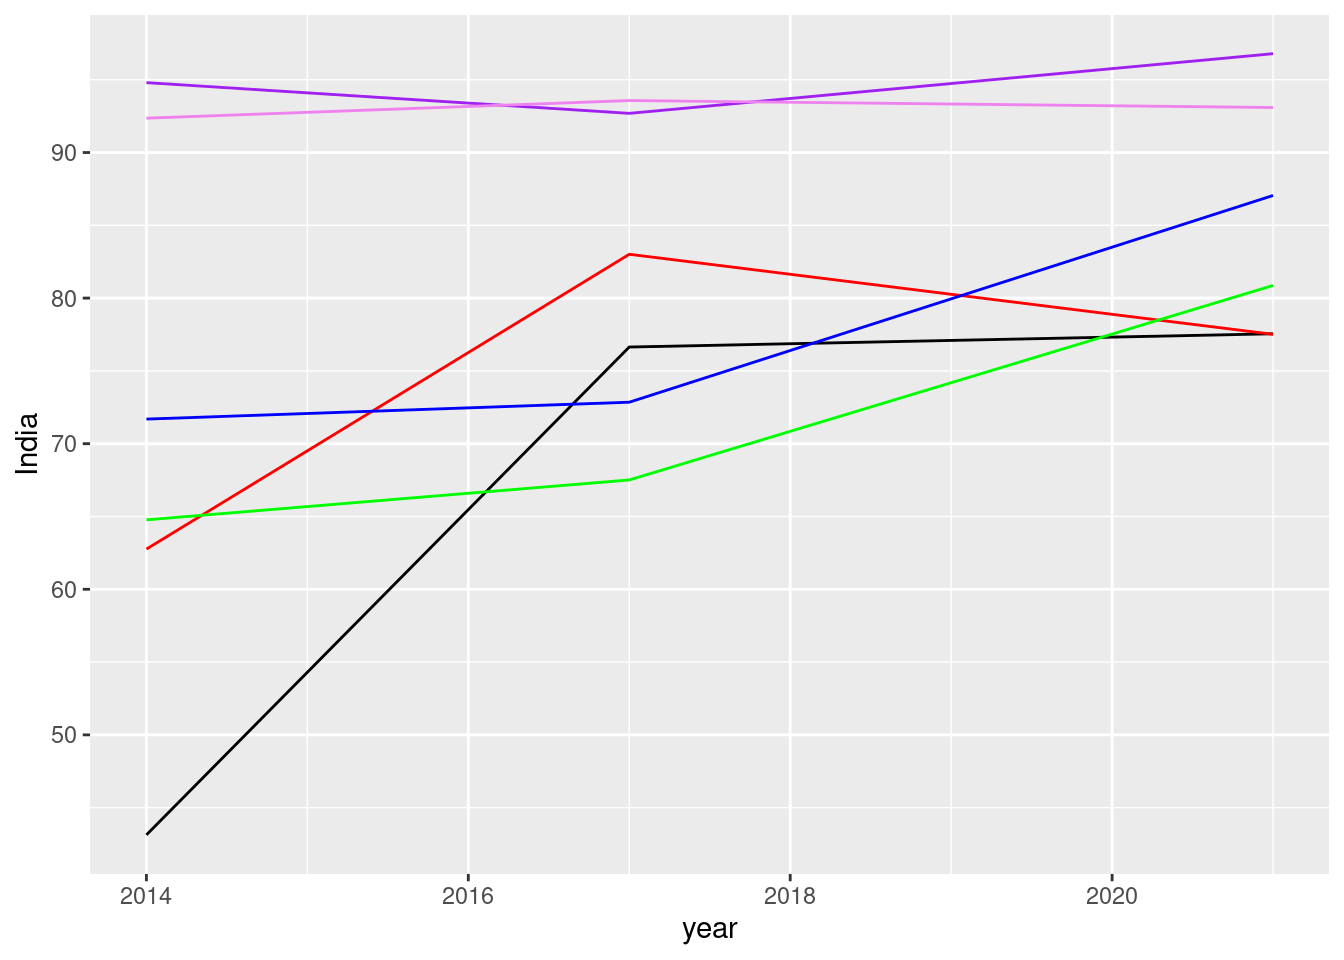
\includegraphics{myproject_files/figure-latex/unnamed-chunk-17-1.pdf}
\textbf{Project 1} i) (Cleaning up the final plot) The final plot is
somewhat misleading: the y-axis is titled ``India''. Write down the code
that will change it to percentage ownership

\begin{Shaded}
\begin{Highlighting}[]
\NormalTok{gfg\_plot }\OtherTok{\textless{}{-}} \FunctionTok{ggplot}\NormalTok{(acct\_owner\_by\_gender, }\FunctionTok{aes}\NormalTok{(}\AttributeTok{x=}\NormalTok{year)) }\SpecialCharTok{+}
\FunctionTok{geom\_line}\NormalTok{(}\FunctionTok{aes}\NormalTok{(}\AttributeTok{y =}\NormalTok{ India), }\AttributeTok{color =} \StringTok{"black"}\NormalTok{) }\SpecialCharTok{+}
\FunctionTok{geom\_line}\NormalTok{(}\FunctionTok{aes}\NormalTok{(}\AttributeTok{y =}\NormalTok{ India\_m), }\AttributeTok{color =} \StringTok{"red"}\NormalTok{) }\SpecialCharTok{+}
\FunctionTok{geom\_line}\NormalTok{(}\FunctionTok{aes}\NormalTok{(}\AttributeTok{y =}\NormalTok{ Brazil), }\AttributeTok{color =} \StringTok{"green"}\NormalTok{) }\SpecialCharTok{+}
\FunctionTok{geom\_line}\NormalTok{(}\FunctionTok{aes}\NormalTok{(}\AttributeTok{y =}\NormalTok{ Brazil\_m), }\AttributeTok{color =} \StringTok{"blue"}\NormalTok{) }\SpecialCharTok{+}
\FunctionTok{geom\_line}\NormalTok{(}\FunctionTok{aes}\NormalTok{(}\AttributeTok{y =}\NormalTok{ United\_States), }\AttributeTok{color =} \StringTok{"purple"}\NormalTok{) }\SpecialCharTok{+}
\FunctionTok{geom\_line}\NormalTok{(}\FunctionTok{aes}\NormalTok{(}\AttributeTok{y =}\NormalTok{ United\_States\_m), }\AttributeTok{color =} \StringTok{"violet"}\NormalTok{) }\SpecialCharTok{+}
\FunctionTok{ylab}\NormalTok{(}\StringTok{"percentage ownership"}\NormalTok{)}
\NormalTok{gfg\_plot}
\end{Highlighting}
\end{Shaded}

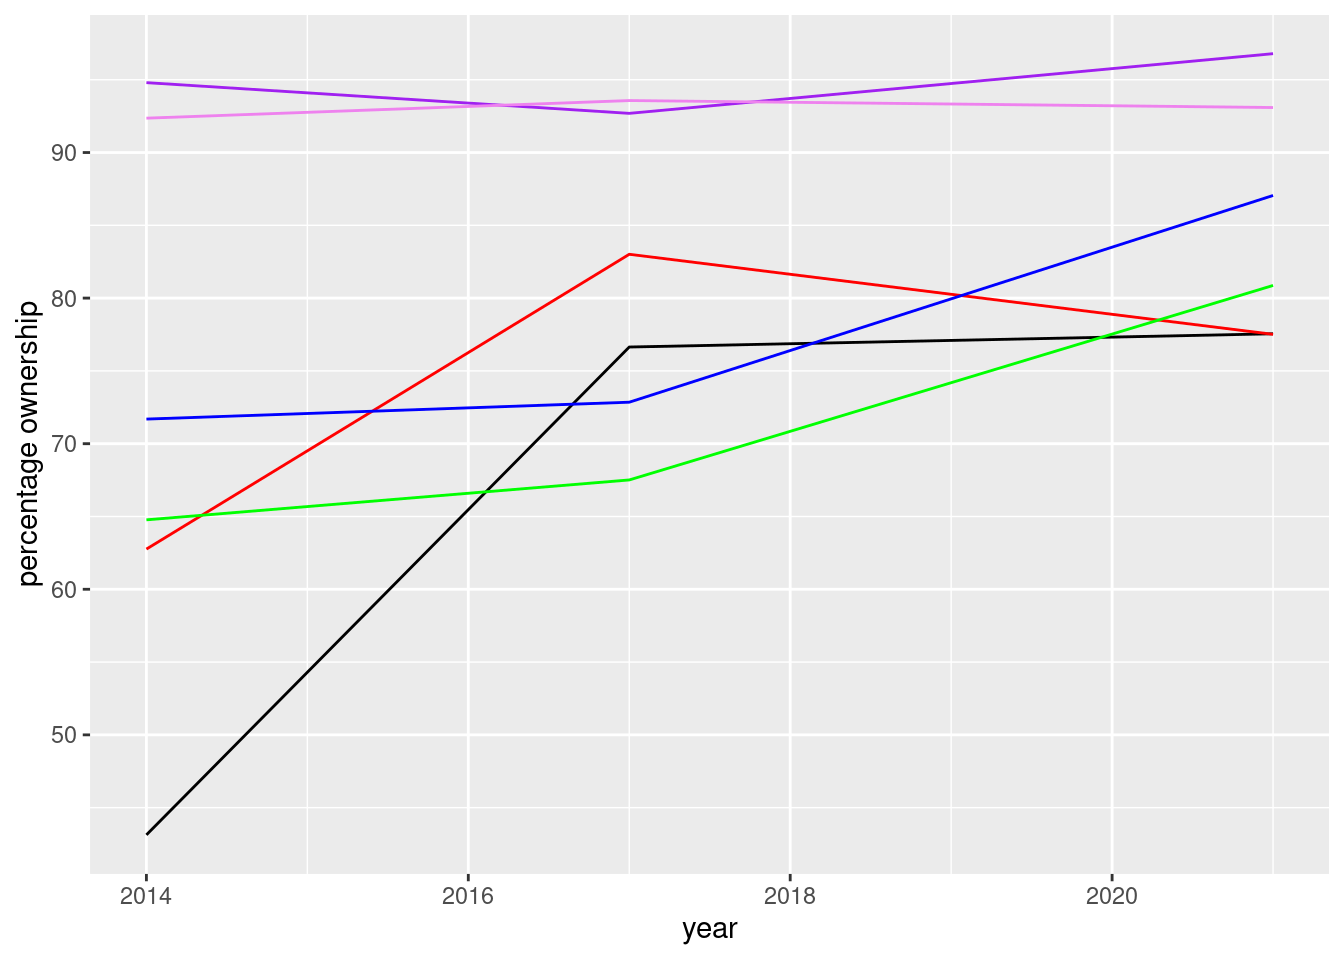
\includegraphics{myproject_files/figure-latex/unnamed-chunk-18-1.pdf}
ii). (Drawing Conclusions) After drawing the plot that includes how
percentages change over time, use this to draw some conclusions on the
how the ownership percentages have been changed. For example, you can
discuss whether males have more account ownership than females and
whether the data suggests that account ownership percentages are on the
rise Conclusions.

-The percentage ownership for males in India was higher than the
percentage ownership for females for the year 2014 to 2020 but
percentage was the same in the year 2021. -The percentage ownership for
males in Brazil was higher than the percentage ownership for females
throughout the years 2014 - 2020 -The percentage ownership for males was
constant throught the years in United States while the percentage
ownership for females was high from 2014 to 2016 declined from 2016 to
2018 then was higher as from 2018. -Generally the average percentage
ownership for both males and females in United states was higher than
those in India and Brazil.

\begin{enumerate}
\def\labelenumi{\roman{enumi})}
\setcounter{enumi}{2}
\tightlist
\item
  (Cherry Picking) Is it possible to say that account percentages have
  been increasing if you disregard a certain year? Does this change if
  you focus on a particular country and gender combinations?
\end{enumerate}

-Generally the account percentages has been increasing over the years.

(Summarizing the data yourself) Do a similar analysis using the csv
files:

\begin{enumerate}
\def\labelenumi{\alph{enumi})}
\tightlist
\item
  Primary data
\end{enumerate}

\begin{Shaded}
\begin{Highlighting}[]
\NormalTok{primary }\OtherTok{\textless{}{-}} \FunctionTok{read.csv}\NormalTok{(}\StringTok{"primary.csv"}\NormalTok{)}
\FunctionTok{head}\NormalTok{(primary)}
\end{Highlighting}
\end{Shaded}

\begin{verbatim}
##                                                                                                                                  Series.Name
## 1 Account ownership at a financial institution or with a mobile-money-service provider, primary education or less (% of population ages 15+)
## 2 Account ownership at a financial institution or with a mobile-money-service provider, primary education or less (% of population ages 15+)
## 3 Account ownership at a financial institution or with a mobile-money-service provider, primary education or less (% of population ages 15+)
## 4 Account ownership at a financial institution or with a mobile-money-service provider, primary education or less (% of population ages 15+)
## 5 Account ownership at a financial institution or with a mobile-money-service provider, primary education or less (% of population ages 15+)
## 6 Account ownership at a financial institution or with a mobile-money-service provider, primary education or less (% of population ages 15+)
##         Series.Code   Country.Name Country.Code X1990..YR1990. X2000..YR2000.
## 1 FX.OWN.TOTL.PL.ZS    Afghanistan          AFG             ..             ..
## 2 FX.OWN.TOTL.PL.ZS        Albania          ALB             ..             ..
## 3 FX.OWN.TOTL.PL.ZS        Algeria          DZA             ..             ..
## 4 FX.OWN.TOTL.PL.ZS American Samoa          ASM             ..             ..
## 5 FX.OWN.TOTL.PL.ZS        Andorra          AND             ..             ..
## 6 FX.OWN.TOTL.PL.ZS         Angola          AGO             ..             ..
##   X2012..YR2012. X2013..YR2013. X2014..YR2014. X2015..YR2015. X2016..YR2016.
## 1             ..             ..           4.83             ..             ..
## 2             ..             ..          24.01             ..             ..
## 3             ..             ..          48.35             ..             ..
## 4             ..             ..             ..             ..             ..
## 5             ..             ..             ..             ..             ..
## 6             ..             ..          14.35             ..             ..
##   X2017..YR2017. X2018..YR2018. X2019..YR2019. X2020..YR2020. X2021..YR2021.
## 1           8.89             ..             ..             ..           5.18
## 2           27.5             ..             ..             ..          34.36
## 3          38.95             ..             ..             ..          38.99
## 4             ..             ..             ..             ..             ..
## 5             ..             ..             ..             ..             ..
## 6             ..             ..             ..             ..             ..
\end{verbatim}

\begin{Shaded}
\begin{Highlighting}[]
\FunctionTok{is.data.frame}\NormalTok{(primary)}
\end{Highlighting}
\end{Shaded}

\begin{verbatim}
## [1] TRUE
\end{verbatim}

\begin{Shaded}
\begin{Highlighting}[]
\NormalTok{primary }\OtherTok{\textless{}{-}}\NormalTok{ primary }\SpecialCharTok{\%\textgreater{}\%}
  \FunctionTok{filter}\NormalTok{(Country.Name }\SpecialCharTok{==} \StringTok{"China"} \SpecialCharTok{|}\NormalTok{ Country.Name }\SpecialCharTok{==} \StringTok{"Israel"} \SpecialCharTok{|}\NormalTok{ Country.Name }\SpecialCharTok{==} \StringTok{"Nigeria"} \SpecialCharTok{|}\NormalTok{ Country.Name }\SpecialCharTok{==} \StringTok{"France"} \SpecialCharTok{|}\NormalTok{ Country.Name }\SpecialCharTok{==} \StringTok{"Algeria"}\NormalTok{)}
\end{Highlighting}
\end{Shaded}

\begin{Shaded}
\begin{Highlighting}[]
\FunctionTok{head}\NormalTok{(primary)}
\end{Highlighting}
\end{Shaded}

\begin{verbatim}
##                                                                                                                                  Series.Name
## 1 Account ownership at a financial institution or with a mobile-money-service provider, primary education or less (% of population ages 15+)
## 2 Account ownership at a financial institution or with a mobile-money-service provider, primary education or less (% of population ages 15+)
## 3 Account ownership at a financial institution or with a mobile-money-service provider, primary education or less (% of population ages 15+)
## 4 Account ownership at a financial institution or with a mobile-money-service provider, primary education or less (% of population ages 15+)
## 5 Account ownership at a financial institution or with a mobile-money-service provider, primary education or less (% of population ages 15+)
##         Series.Code Country.Name Country.Code X1990..YR1990. X2000..YR2000.
## 1 FX.OWN.TOTL.PL.ZS      Algeria          DZA             ..             ..
## 2 FX.OWN.TOTL.PL.ZS        China          CHN             ..             ..
## 3 FX.OWN.TOTL.PL.ZS       France          FRA             ..             ..
## 4 FX.OWN.TOTL.PL.ZS       Israel          ISR             ..             ..
## 5 FX.OWN.TOTL.PL.ZS      Nigeria          NGA             ..             ..
##   X2012..YR2012. X2013..YR2013. X2014..YR2014. X2015..YR2015. X2016..YR2016.
## 1             ..             ..          48.35             ..             ..
## 2             ..             ..          72.82             ..             ..
## 3             ..             ..          83.36             ..             ..
## 4             ..             ..          83.69             ..             ..
## 5             ..             ..          28.08             ..             ..
##   X2017..YR2017. X2018..YR2018. X2019..YR2019. X2020..YR2020. X2021..YR2021.
## 1          38.95             ..             ..             ..          38.99
## 2          71.39             ..             ..             ..          83.02
## 3          79.82             ..             ..             ..          95.87
## 4          88.29             ..             ..             ..          62.76
## 5          16.05             ..             ..             ..           25.8
\end{verbatim}

\begin{Shaded}
\begin{Highlighting}[]
\CommentTok{\# Drop unnecessary columns}
\NormalTok{primary }\OtherTok{\textless{}{-}}\NormalTok{ primary[ }\SpecialCharTok{{-}}\FunctionTok{c}\NormalTok{(}\DecValTok{1}\NormalTok{,}\DecValTok{2}\NormalTok{,}\DecValTok{4}\NormalTok{,}\DecValTok{5}\SpecialCharTok{:}\DecValTok{8}\NormalTok{,}\DecValTok{10}\SpecialCharTok{:}\DecValTok{11}\NormalTok{,}\DecValTok{13}\SpecialCharTok{:}\DecValTok{15}\NormalTok{)] }\SpecialCharTok{\%\textgreater{}\%}
  \FunctionTok{rename}\NormalTok{(}\StringTok{"2014"} \OtherTok{=} \DecValTok{2}\NormalTok{, }\StringTok{"2017"} \OtherTok{=} \DecValTok{3}\NormalTok{, }\StringTok{"2021"} \OtherTok{=} \DecValTok{4}\NormalTok{)}

\FunctionTok{head}\NormalTok{(primary)}
\end{Highlighting}
\end{Shaded}

\begin{verbatim}
##   Country.Name  2014  2017  2021
## 1      Algeria 48.35 38.95 38.99
## 2        China 72.82 71.39 83.02
## 3       France 83.36 79.82 95.87
## 4       Israel 83.69 88.29 62.76
## 5      Nigeria 28.08 16.05  25.8
\end{verbatim}

\begin{Shaded}
\begin{Highlighting}[]
\NormalTok{transpose\_p }\OtherTok{\textless{}{-}} \FunctionTok{data.frame}\NormalTok{(}\FunctionTok{t}\NormalTok{(primary[}\SpecialCharTok{{-}}\DecValTok{1}\NormalTok{]))}
\FunctionTok{colnames}\NormalTok{(transpose\_p) }\OtherTok{\textless{}{-}}\NormalTok{ primary[, }\DecValTok{1}\NormalTok{]}

\FunctionTok{head}\NormalTok{(transpose\_p)}
\end{Highlighting}
\end{Shaded}

\begin{verbatim}
##      Algeria China France Israel Nigeria
## 2014   48.35 72.82  83.36  83.69   28.08
## 2017   38.95 71.39  79.82  88.29   16.05
## 2021   38.99 83.02  95.87  62.76    25.8
\end{verbatim}

\begin{Shaded}
\begin{Highlighting}[]
\FunctionTok{print}\NormalTok{(}\FunctionTok{sapply}\NormalTok{(transpose\_p, class))}
\end{Highlighting}
\end{Shaded}

\begin{verbatim}
##     Algeria       China      France      Israel     Nigeria 
## "character" "character" "character" "character" "character"
\end{verbatim}

\begin{Shaded}
\begin{Highlighting}[]
\CommentTok{\# converting the character values to numeric}
\NormalTok{transpose\_p}\SpecialCharTok{$}\NormalTok{Algeria }\OtherTok{=} \FunctionTok{as.numeric}\NormalTok{(}\FunctionTok{as.character}\NormalTok{(transpose\_p}\SpecialCharTok{$}\NormalTok{Algeria))}
\NormalTok{transpose\_p}\SpecialCharTok{$}\NormalTok{China }\OtherTok{=} \FunctionTok{as.numeric}\NormalTok{(}\FunctionTok{as.character}\NormalTok{(transpose\_p}\SpecialCharTok{$}\NormalTok{China))}
\NormalTok{transpose\_p}\SpecialCharTok{$}\NormalTok{Nigeria }\OtherTok{=} \FunctionTok{as.numeric}\NormalTok{(}\FunctionTok{as.character}\NormalTok{(transpose\_p}\SpecialCharTok{$}\NormalTok{Nigeria))}
\NormalTok{transpose\_p}\SpecialCharTok{$}\NormalTok{France }\OtherTok{=} \FunctionTok{as.numeric}\NormalTok{(}\FunctionTok{as.character}\NormalTok{(transpose\_p}\SpecialCharTok{$}\NormalTok{France))}
\NormalTok{transpose\_p}\SpecialCharTok{$}\NormalTok{Israel }\OtherTok{=} \FunctionTok{as.numeric}\NormalTok{(}\FunctionTok{as.character}\NormalTok{(transpose\_p}\SpecialCharTok{$}\NormalTok{Israel))}


\FunctionTok{head}\NormalTok{(transpose\_p)}
\end{Highlighting}
\end{Shaded}

\begin{verbatim}
##      Algeria China France Israel Nigeria
## 2014   48.35 72.82  83.36  83.69   28.08
## 2017   38.95 71.39  79.82  88.29   16.05
## 2021   38.99 83.02  95.87  62.76   25.80
\end{verbatim}

\begin{Shaded}
\begin{Highlighting}[]
\CommentTok{\#Summary of each category}
\FunctionTok{summarise\_each}\NormalTok{(transpose\_p, }\FunctionTok{list}\NormalTok{(mean))}
\end{Highlighting}
\end{Shaded}

\begin{verbatim}
##    Algeria    China France   Israel Nigeria
## 1 42.09667 75.74333  86.35 78.24667   23.31
\end{verbatim}

\begin{Shaded}
\begin{Highlighting}[]
\NormalTok{year }\OtherTok{\textless{}{-}} \FunctionTok{c}\NormalTok{(}\DecValTok{2014}\NormalTok{, }\DecValTok{2017}\NormalTok{, }\DecValTok{2021}\NormalTok{)}

\FunctionTok{ggplot}\NormalTok{(}\AttributeTok{data =}\NormalTok{ transpose\_p, }\FunctionTok{aes}\NormalTok{(}\AttributeTok{x=}\NormalTok{year, }\AttributeTok{y=}\NormalTok{China, }\AttributeTok{group =} \DecValTok{1}\NormalTok{)) }\SpecialCharTok{+}
  \FunctionTok{geom\_line}\NormalTok{() }\SpecialCharTok{+}
  \FunctionTok{geom\_point}\NormalTok{()}
\end{Highlighting}
\end{Shaded}

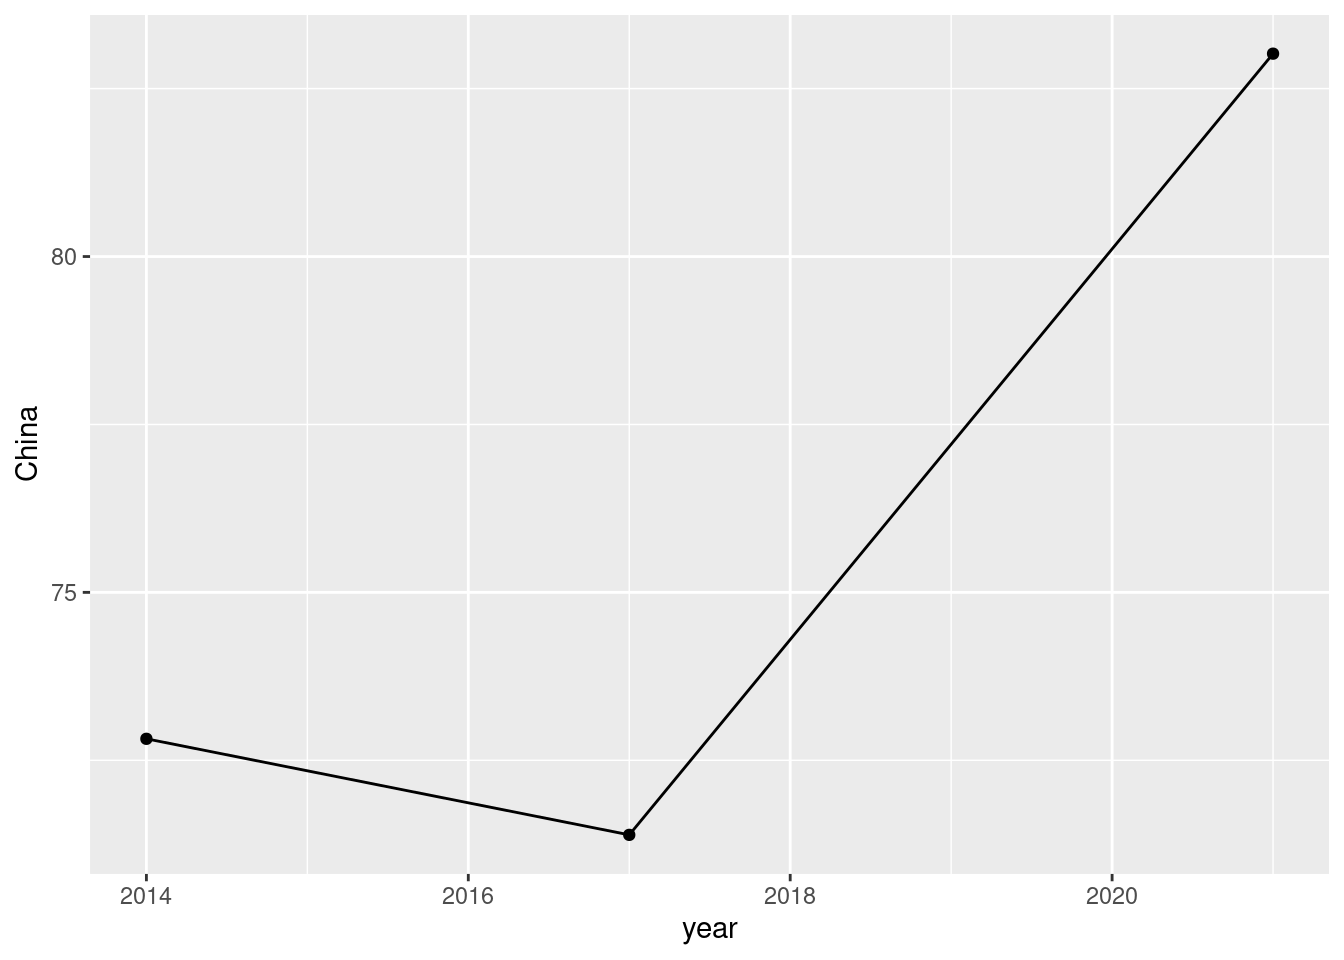
\includegraphics{myproject_files/figure-latex/unnamed-chunk-28-1.pdf}
Merging the two datasets together

\begin{Shaded}
\begin{Highlighting}[]
\NormalTok{secondary }\OtherTok{\textless{}{-}} \FunctionTok{read.csv}\NormalTok{(}\AttributeTok{file =} \StringTok{"secondary.csv"}\NormalTok{)}

\NormalTok{secondary }\OtherTok{\textless{}{-}}\NormalTok{ secondary }\SpecialCharTok{\%\textgreater{}\%}
  \FunctionTok{filter}\NormalTok{(Country.Name }\SpecialCharTok{==} \StringTok{"China"} \SpecialCharTok{|}\NormalTok{ Country.Name }\SpecialCharTok{==} \StringTok{"Israel"} \SpecialCharTok{|}\NormalTok{ Country.Name }\SpecialCharTok{==} \StringTok{"Nigeria"} \SpecialCharTok{|}\NormalTok{ Country.Name }\SpecialCharTok{==} \StringTok{"France"} \SpecialCharTok{|}\NormalTok{ Country.Name }\SpecialCharTok{==} \StringTok{"Algeria"}\NormalTok{)}

\NormalTok{secondary }\OtherTok{\textless{}{-}}\NormalTok{ secondary[ }\SpecialCharTok{{-}}\FunctionTok{c}\NormalTok{(}\DecValTok{1}\NormalTok{,}\DecValTok{2}\NormalTok{,}\DecValTok{4}\NormalTok{,}\DecValTok{5}\SpecialCharTok{:}\DecValTok{8}\NormalTok{,}\DecValTok{10}\SpecialCharTok{:}\DecValTok{11}\NormalTok{,}\DecValTok{13}\SpecialCharTok{:}\DecValTok{15}\NormalTok{)] }\SpecialCharTok{\%\textgreater{}\%}
\FunctionTok{rename}\NormalTok{(}\StringTok{"2014"} \OtherTok{=} \DecValTok{2}\NormalTok{, }\StringTok{"2017"} \OtherTok{=} \DecValTok{3}\NormalTok{, }\StringTok{"2021"} \OtherTok{=} \DecValTok{4}\NormalTok{)}


\NormalTok{transpose\_s }\OtherTok{\textless{}{-}} \FunctionTok{data.frame}\NormalTok{(}\FunctionTok{t}\NormalTok{(secondary[}\SpecialCharTok{{-}}\DecValTok{1}\NormalTok{]))}
\FunctionTok{colnames}\NormalTok{(transpose\_s) }\OtherTok{\textless{}{-}}\NormalTok{ secondary[, }\DecValTok{1}\NormalTok{]}

\CommentTok{\# converting the character values to numeric}
\NormalTok{transpose\_s}\SpecialCharTok{$}\NormalTok{Algeria }\OtherTok{=} \FunctionTok{as.numeric}\NormalTok{(}\FunctionTok{as.character}\NormalTok{(transpose\_s}\SpecialCharTok{$}\NormalTok{Algeria))}
\NormalTok{transpose\_s}\SpecialCharTok{$}\NormalTok{China }\OtherTok{=} \FunctionTok{as.numeric}\NormalTok{(}\FunctionTok{as.character}\NormalTok{(transpose\_s}\SpecialCharTok{$}\NormalTok{China))}
\NormalTok{transpose\_s}\SpecialCharTok{$}\NormalTok{Nigeria }\OtherTok{=} \FunctionTok{as.numeric}\NormalTok{(}\FunctionTok{as.character}\NormalTok{(transpose\_s}\SpecialCharTok{$}\NormalTok{Nigeria))}
\NormalTok{transpose\_s}\SpecialCharTok{$}\NormalTok{France }\OtherTok{=} \FunctionTok{as.numeric}\NormalTok{(}\FunctionTok{as.character}\NormalTok{(transpose\_s}\SpecialCharTok{$}\NormalTok{France))}
\NormalTok{transpose\_s}\SpecialCharTok{$}\NormalTok{Israel }\OtherTok{=} \FunctionTok{as.numeric}\NormalTok{(}\FunctionTok{as.character}\NormalTok{(transpose\_s}\SpecialCharTok{$}\NormalTok{Israel))}
\end{Highlighting}
\end{Shaded}

\begin{Shaded}
\begin{Highlighting}[]
\FunctionTok{head}\NormalTok{(transpose\_s)}
\end{Highlighting}
\end{Shaded}

\begin{verbatim}
##      Algeria China France Israel Nigeria
## 2014   55.32 89.84  97.26  90.17   56.03
## 2017   48.96 94.14  97.23  93.01   59.30
## 2021   46.23 97.21  99.76  94.27   65.20
\end{verbatim}

\begin{Shaded}
\begin{Highlighting}[]
\NormalTok{transpose\_s }\OtherTok{\textless{}{-}} \FunctionTok{rename}\NormalTok{(transpose\_s, }\StringTok{"Algeria\_s"} \OtherTok{=} \DecValTok{1}\NormalTok{, }\StringTok{"China\_s"} \OtherTok{=} \DecValTok{2}\NormalTok{, }\StringTok{"France\_s"} \OtherTok{=} \DecValTok{3}\NormalTok{, }\StringTok{"Israel\_s"} \OtherTok{=} \DecValTok{4}\NormalTok{, }\StringTok{"Nigeria\_s"} \OtherTok{=} \DecValTok{5}\NormalTok{)}

\FunctionTok{head}\NormalTok{(transpose\_s)}
\end{Highlighting}
\end{Shaded}

\begin{verbatim}
##      Algeria_s China_s France_s Israel_s Nigeria_s
## 2014     55.32   89.84    97.26    90.17     56.03
## 2017     48.96   94.14    97.23    93.01     59.30
## 2021     46.23   97.21    99.76    94.27     65.20
\end{verbatim}

\begin{Shaded}
\begin{Highlighting}[]
\NormalTok{transpose\_p }\OtherTok{\textless{}{-}} \FunctionTok{rownames\_to\_column}\NormalTok{(transpose\_p, }\AttributeTok{var=}\StringTok{"Year"}\NormalTok{)}
\NormalTok{transpose\_s }\OtherTok{\textless{}{-}} \FunctionTok{rownames\_to\_column}\NormalTok{(transpose\_s, }\AttributeTok{var=}\StringTok{"Year"}\NormalTok{)}
\end{Highlighting}
\end{Shaded}

\begin{Shaded}
\begin{Highlighting}[]
\NormalTok{acct\_owner\_by\_lev\_educ }\OtherTok{\textless{}{-}} \FunctionTok{merge}\NormalTok{(}\AttributeTok{x =}\NormalTok{ transpose\_s, }\AttributeTok{y=}\NormalTok{transpose\_p, }\AttributeTok{by =}\StringTok{"Year"}\NormalTok{, }\AttributeTok{all.x =} \ConstantTok{TRUE}\NormalTok{)}

\FunctionTok{head}\NormalTok{(acct\_owner\_by\_lev\_educ)}
\end{Highlighting}
\end{Shaded}

\begin{verbatim}
##   Year Algeria_s China_s France_s Israel_s Nigeria_s Algeria China France
## 1 2014     55.32   89.84    97.26    90.17     56.03   48.35 72.82  83.36
## 2 2017     48.96   94.14    97.23    93.01     59.30   38.95 71.39  79.82
## 3 2021     46.23   97.21    99.76    94.27     65.20   38.99 83.02  95.87
##   Israel Nigeria
## 1  83.69   28.08
## 2  88.29   16.05
## 3  62.76   25.80
\end{verbatim}

\begin{Shaded}
\begin{Highlighting}[]
\NormalTok{gfg\_plot }\OtherTok{\textless{}{-}} \FunctionTok{ggplot}\NormalTok{(acct\_owner\_by\_lev\_educ, }\FunctionTok{aes}\NormalTok{(}\AttributeTok{x=}\NormalTok{year)) }\SpecialCharTok{+}
\FunctionTok{geom\_line}\NormalTok{(}\FunctionTok{aes}\NormalTok{(}\AttributeTok{y =}\NormalTok{ Nigeria), }\AttributeTok{color =} \StringTok{"black"}\NormalTok{) }\SpecialCharTok{+}
\FunctionTok{geom\_line}\NormalTok{(}\FunctionTok{aes}\NormalTok{(}\AttributeTok{y =}\NormalTok{ Nigeria\_s), }\AttributeTok{color =} \StringTok{"red"}\NormalTok{) }\SpecialCharTok{+}
\FunctionTok{geom\_line}\NormalTok{(}\FunctionTok{aes}\NormalTok{(}\AttributeTok{y =}\NormalTok{ China), }\AttributeTok{color =} \StringTok{"green"}\NormalTok{) }\SpecialCharTok{+}
\FunctionTok{geom\_line}\NormalTok{(}\FunctionTok{aes}\NormalTok{(}\AttributeTok{y =}\NormalTok{ China\_s), }\AttributeTok{color =} \StringTok{"blue"}\NormalTok{) }\SpecialCharTok{+}
\FunctionTok{geom\_line}\NormalTok{(}\FunctionTok{aes}\NormalTok{(}\AttributeTok{y =}\NormalTok{ France), }\AttributeTok{color =} \StringTok{"purple"}\NormalTok{) }\SpecialCharTok{+}
\FunctionTok{geom\_line}\NormalTok{(}\FunctionTok{aes}\NormalTok{(}\AttributeTok{y =}\NormalTok{ France\_s), }\AttributeTok{color =} \StringTok{"violet"}\NormalTok{)}\SpecialCharTok{+}
\FunctionTok{geom\_line}\NormalTok{(}\FunctionTok{aes}\NormalTok{(}\AttributeTok{y =}\NormalTok{ Algeria), }\AttributeTok{color =} \StringTok{"yellow"}\NormalTok{) }\SpecialCharTok{+}
\FunctionTok{geom\_line}\NormalTok{(}\FunctionTok{aes}\NormalTok{(}\AttributeTok{y =}\NormalTok{ Algeria\_s), }\AttributeTok{color =} \StringTok{"brown"}\NormalTok{) }\SpecialCharTok{+}
\FunctionTok{geom\_line}\NormalTok{(}\FunctionTok{aes}\NormalTok{(}\AttributeTok{y =}\NormalTok{ Israel), }\AttributeTok{color =} \StringTok{"pink"}\NormalTok{)}\SpecialCharTok{+}
\FunctionTok{geom\_line}\NormalTok{(}\FunctionTok{aes}\NormalTok{(}\AttributeTok{y =}\NormalTok{ Israel\_s), }\AttributeTok{color =} \StringTok{"gray"}\NormalTok{)}\SpecialCharTok{+}
  \FunctionTok{ylab}\NormalTok{(}\StringTok{"Percentage Ownership"}\NormalTok{)}

\NormalTok{gfg\_plot}
\end{Highlighting}
\end{Shaded}

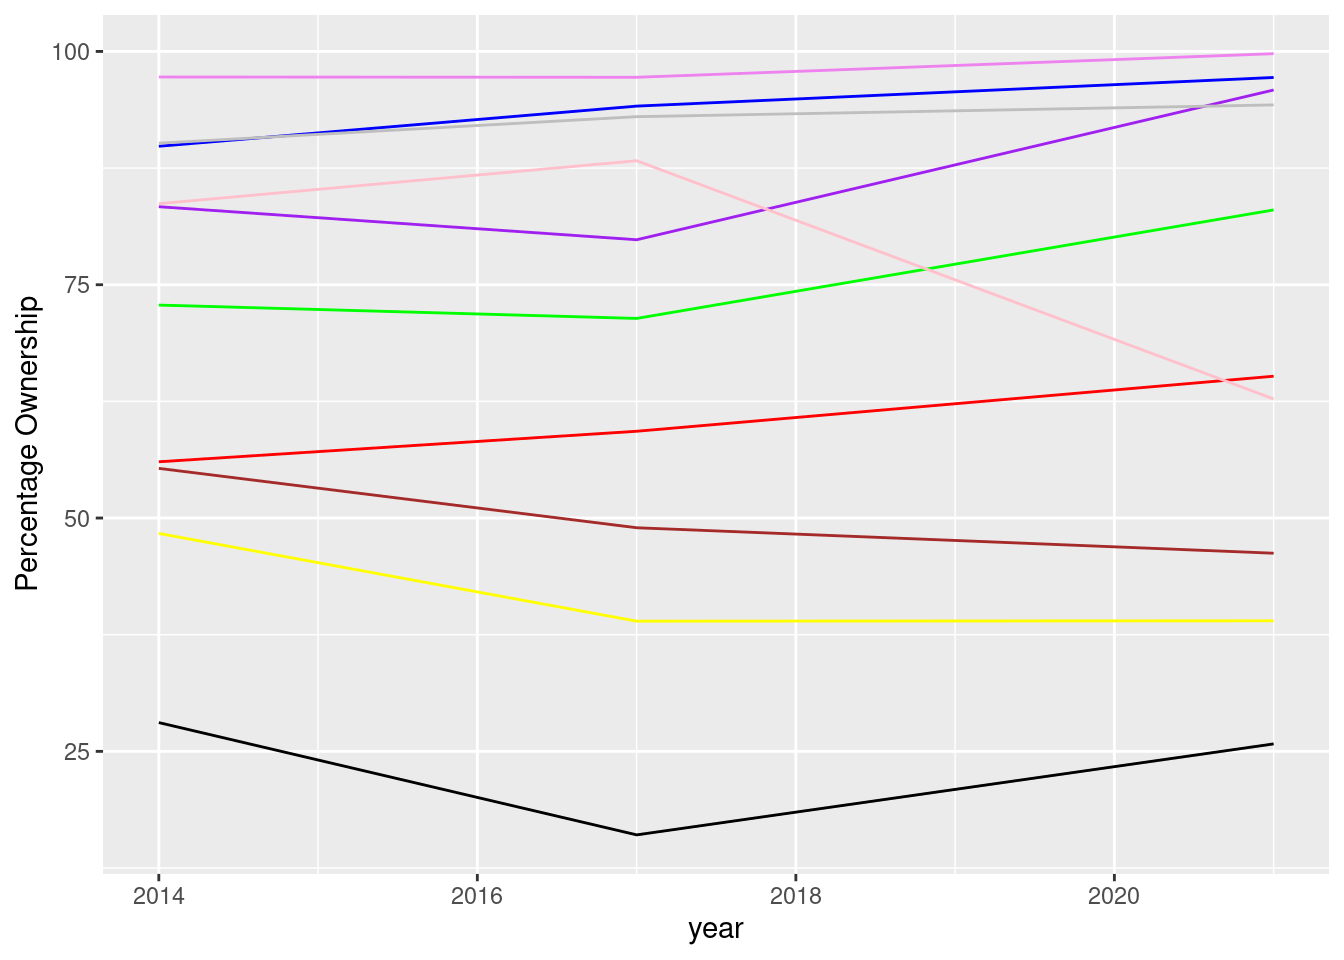
\includegraphics{myproject_files/figure-latex/unnamed-chunk-34-1.pdf}
Conclusions. -Generally the percentage ownership of students in
secondary is higher than the percentage ownership of students in
primary. - The percentage ownership for Secondary students in France is
higher the percentage ownership in other countries. -The percentage
ownership for primary students in Nigeria was the lowest compared to
other countries.

Project Two

\begin{Shaded}
\begin{Highlighting}[]
\FunctionTok{set.seed}\NormalTok{(}\DecValTok{1}\NormalTok{)}
\NormalTok{coin\_flips }\OtherTok{\textless{}{-}} \FunctionTok{rbinom}\NormalTok{(}\DecValTok{100}\NormalTok{, }\DecValTok{1}\NormalTok{, .}\DecValTok{5}\NormalTok{)}
\NormalTok{coin\_flips}
\end{Highlighting}
\end{Shaded}

\begin{verbatim}
##   [1] 0 0 1 1 0 1 1 1 1 0 0 0 1 0 1 0 1 1 0 1 1 0 1 0 0 0 0 0 1 0 0 1 0 0 1 1 1
##  [38] 0 1 0 1 1 1 1 1 1 0 0 1 1 0 1 0 0 0 0 0 1 1 0 1 0 0 0 1 0 0 1 0 1 0 1 0 0
##  [75] 0 1 1 0 1 1 0 1 0 0 1 0 1 0 0 0 0 0 1 1 1 1 0 0 1 1
\end{verbatim}

\begin{Shaded}
\begin{Highlighting}[]
\NormalTok{Data }\OtherTok{\textless{}{-}} \FunctionTok{data.frame}\NormalTok{(}\AttributeTok{toss\_number =}\NormalTok{ (}\DecValTok{1}\SpecialCharTok{:}\FunctionTok{length}\NormalTok{(coin\_flips)), }\AttributeTok{toss\_result =}\NormalTok{ coin\_flips)}

\FunctionTok{head}\NormalTok{(Data, }\DecValTok{5}\NormalTok{)}
\end{Highlighting}
\end{Shaded}

\begin{verbatim}
##   toss_number toss_result
## 1           1           0
## 2           2           0
## 3           3           1
## 4           4           1
## 5           5           0
\end{verbatim}

\begin{Shaded}
\begin{Highlighting}[]
\NormalTok{frequencies }\OtherTok{\textless{}{-}} \ControlFlowTok{function}\NormalTok{(vec)\{}
\NormalTok{  len\_vec }\OtherTok{\textless{}{-}} \FunctionTok{length}\NormalTok{(vec)}
  
\NormalTok{  avg }\OtherTok{\textless{}{-}} \DecValTok{1}\SpecialCharTok{:}\NormalTok{len\_vec}
  
  \ControlFlowTok{for}\NormalTok{ (i }\ControlFlowTok{in} \DecValTok{1}\SpecialCharTok{:}\NormalTok{len\_vec)\{}
\NormalTok{    avg[i] }\OtherTok{\textless{}{-}} \FunctionTok{length}\NormalTok{(}\FunctionTok{which}\NormalTok{(vec[}\DecValTok{1}\SpecialCharTok{:}\NormalTok{i] }\SpecialCharTok{==} \DecValTok{1}\NormalTok{)) }\SpecialCharTok{/}\NormalTok{ i}
\NormalTok{  \}}
  \FunctionTok{return}\NormalTok{(avg)}
\NormalTok{\}}

\NormalTok{freq }\OtherTok{\textless{}{-}} \FunctionTok{frequencies}\NormalTok{(coin\_flips)}
\NormalTok{Data}\SpecialCharTok{$}\NormalTok{avgs }\OtherTok{\textless{}{-}}\NormalTok{ freq}
\FunctionTok{head}\NormalTok{(Data, }\DecValTok{5}\NormalTok{)}
\end{Highlighting}
\end{Shaded}

\begin{verbatim}
##   toss_number toss_result      avgs
## 1           1           0 0.0000000
## 2           2           0 0.0000000
## 3           3           1 0.3333333
## 4           4           1 0.5000000
## 5           5           0 0.4000000
\end{verbatim}

\begin{Shaded}
\begin{Highlighting}[]
\NormalTok{estimate\_pi }\OtherTok{\textless{}{-}} \ControlFlowTok{function}\NormalTok{(}\AttributeTok{seed =}\DecValTok{1}\NormalTok{, }\AttributeTok{iterations =} \DecValTok{10000}\NormalTok{) \{}
  \FunctionTok{set.seed}\NormalTok{(seed)}
  
\NormalTok{  x }\OtherTok{\textless{}{-}} \FunctionTok{runif}\NormalTok{(}\AttributeTok{n =}\NormalTok{ iterations, }\AttributeTok{min =} \DecValTok{0}\NormalTok{, }\AttributeTok{max =} \DecValTok{1}\NormalTok{)}
  
\NormalTok{  val\_of\_g }\OtherTok{=} \FunctionTok{sqrt}\NormalTok{(}\DecValTok{1}\SpecialCharTok{{-}}\NormalTok{x}\SpecialCharTok{\^{}}\DecValTok{2}\NormalTok{)}
  
\NormalTok{  pi\_over\_four }\OtherTok{=} \FunctionTok{mean}\NormalTok{(val\_of\_g)}
  
\NormalTok{  pi }\OtherTok{\textless{}{-}} \DecValTok{4} \SpecialCharTok{*}\NormalTok{pi\_over\_four}
  
  \FunctionTok{return}\NormalTok{(pi)}
  
\NormalTok{\}}
\end{Highlighting}
\end{Shaded}

\begin{Shaded}
\begin{Highlighting}[]
\FunctionTok{estimate\_pi}\NormalTok{()}
\end{Highlighting}
\end{Shaded}

\begin{verbatim}
## [1] 3.134608
\end{verbatim}

\hypertarget{project-2}{%
\section{Project 2:}\label{project-2}}

\begin{enumerate}
\def\labelenumi{\arabic{enumi}.}
\tightlist
\item
  Consider an experiment where you toss a a fair coin 12 times. Let X be
  the number of heads that you obtain. Note that X ∼ Bin(12, 1/2).
\end{enumerate}

\begin{enumerate}
\def\labelenumi{(\alph{enumi})}
\tightlist
\item
  Compute P(X = 7) (using the formulas associated with the binomial
  distributions. R can compute the theoretical value as well if you
  choose to go that route)
\end{enumerate}

\begin{Shaded}
\begin{Highlighting}[]
\FunctionTok{set.seed}\NormalTok{(}\DecValTok{23}\NormalTok{)}
\NormalTok{coin }\OtherTok{\textless{}{-}} \FunctionTok{dbinom}\NormalTok{(}\DecValTok{7}\NormalTok{, }\DecValTok{12}\NormalTok{, }\FloatTok{0.5}\NormalTok{)}

\NormalTok{coin}
\end{Highlighting}
\end{Shaded}

\begin{verbatim}
## [1] 0.1933594
\end{verbatim}

\begin{enumerate}
\def\labelenumi{(\alph{enumi})}
\setcounter{enumi}{1}
\tightlist
\item
  Plot the evolution of the relative frequency for X = 7 based on
  1000000 repetitions of the above.
\end{enumerate}

\begin{Shaded}
\begin{Highlighting}[]
\FunctionTok{set.seed}\NormalTok{(}\DecValTok{23}\NormalTok{)}
\NormalTok{num\_reps }\OtherTok{\textless{}{-}} \DecValTok{1000000}
\NormalTok{X\_7 }\OtherTok{\textless{}{-}} \FunctionTok{rep}\NormalTok{(}\ConstantTok{NA}\NormalTok{, num\_reps)}

\ControlFlowTok{for}\NormalTok{(i }\ControlFlowTok{in} \DecValTok{1}\SpecialCharTok{:}\NormalTok{num\_reps) \{}
\NormalTok{  coin\_flips }\OtherTok{\textless{}{-}} \FunctionTok{rbinom}\NormalTok{(}\DecValTok{12}\NormalTok{, }\DecValTok{1}\NormalTok{, }\FloatTok{0.5}\NormalTok{)}
\NormalTok{  X\_7[i] }\OtherTok{\textless{}{-}} \FunctionTok{sum}\NormalTok{(coin\_flips }\SpecialCharTok{==} \DecValTok{1}\NormalTok{)}
\NormalTok{\}}

\NormalTok{rel\_freqs }\OtherTok{\textless{}{-}} \FunctionTok{cumsum}\NormalTok{(X\_7 }\SpecialCharTok{==} \DecValTok{7}\NormalTok{) }\SpecialCharTok{/} \FunctionTok{seq\_along}\NormalTok{(X\_7)}

\FunctionTok{ggplot}\NormalTok{(}\AttributeTok{data =} \FunctionTok{data.frame}\NormalTok{(}\AttributeTok{trial =} \DecValTok{1}\SpecialCharTok{:}\NormalTok{num\_reps, }\AttributeTok{relative\_frequency =}\NormalTok{ rel\_freqs), }\FunctionTok{aes}\NormalTok{(}\AttributeTok{x =}\NormalTok{ trial, }\AttributeTok{y =}\NormalTok{ relative\_frequency)) }\SpecialCharTok{+}
  \FunctionTok{geom\_line}\NormalTok{() }\SpecialCharTok{+}
  \FunctionTok{labs}\NormalTok{(}\AttributeTok{x =} \StringTok{"Trial"}\NormalTok{, }\AttributeTok{y =} \StringTok{"Relative Frequency"}\NormalTok{)}
\end{Highlighting}
\end{Shaded}

\includegraphics{myproject_files/figure-latex/unnamed-chunk-41-1.pdf} c)
Explain how your observations match up with the frequentist
interpretation of probability.

The frequentist interpretation of probability states that the
probability of an event is the limit of the relative frequency of that
event as the number of repetitions of the experiment approaches
infinity. In our case, as we increase the number of repetitions of the
experiment (i.e., the number of times we toss the coin 12 times), we
observe that the relative frequency of obtaining 7 heads approaches the
theoretical probability of P(X = 7). This is consistent with the
frequentist interpretation of probability.

\begin{enumerate}
\def\labelenumi{\alph{enumi})}
\setcounter{enumi}{3}
\tightlist
\item
  Compute E(X) and the observed average of the repetitions
\end{enumerate}

The expected value of X is given by E(X) = np = 12 * 0.5 = 6

\begin{Shaded}
\begin{Highlighting}[]
\FunctionTok{mean}\NormalTok{(X\_7)}
\end{Highlighting}
\end{Shaded}

\begin{verbatim}
## [1] 6.000366
\end{verbatim}

\begin{enumerate}
\def\labelenumi{\alph{enumi})}
\setcounter{enumi}{4}
\tightlist
\item
  Do your observations match up with the law of large numbers?
\end{enumerate}

The law of large numbers states that as the number of repetitions of an
experiment increases, the sample mean approaches the true mean of the
population. In our case, as we increase the number of repetitions of the
experiment, we observe that the observed average of the repetitions
approaches the expected value of X, which is consistent with the law of
large numbers.

\begin{enumerate}
\def\labelenumi{\arabic{enumi}.}
\setcounter{enumi}{1}
\tightlist
\item
  Experimentally verify the law of large numbers for the standard normal
  distribution and an exponential distribution with λ = 4
\end{enumerate}

For the standard normal distribution, the law of large numbers states
that the sample mean of a large number of independent and identically
distributed normal random variables will converge to the population
mean. Similarly, for an exponential distribution with parameter λ, the
sample mean will converge to the population mean 1/λ

For the standard distribution

\begin{Shaded}
\begin{Highlighting}[]
\FunctionTok{set.seed}\NormalTok{(}\DecValTok{1}\NormalTok{)}
\NormalTok{n }\OtherTok{\textless{}{-}} \FunctionTok{c}\NormalTok{(}\DecValTok{10}\NormalTok{, }\DecValTok{100}\NormalTok{, }\DecValTok{1000}\NormalTok{, }\DecValTok{10000}\NormalTok{, }\DecValTok{100000}\NormalTok{)}

\ControlFlowTok{for}\NormalTok{ (i }\ControlFlowTok{in}\NormalTok{ n) \{}
\NormalTok{  x }\OtherTok{\textless{}{-}} \FunctionTok{rnorm}\NormalTok{(i)}
  \FunctionTok{print}\NormalTok{(}\FunctionTok{mean}\NormalTok{(x))}
\NormalTok{\}}
\end{Highlighting}
\end{Shaded}

\begin{verbatim}
## [1] 0.1322028
## [1] 0.1304151
## [1] -0.02765614
## [1] -0.006409792
## [1] -0.001154808
\end{verbatim}

For the Exponential Distribution

\begin{Shaded}
\begin{Highlighting}[]
\FunctionTok{set.seed}\NormalTok{(}\DecValTok{1}\NormalTok{)}
\NormalTok{n }\OtherTok{\textless{}{-}} \FunctionTok{c}\NormalTok{(}\DecValTok{10}\NormalTok{, }\DecValTok{100}\NormalTok{, }\DecValTok{1000}\NormalTok{, }\DecValTok{10000}\NormalTok{, }\DecValTok{100000}\NormalTok{)}

\ControlFlowTok{for}\NormalTok{ (i }\ControlFlowTok{in}\NormalTok{ n) \{}
\NormalTok{  x }\OtherTok{\textless{}{-}} \FunctionTok{rexp}\NormalTok{(i, }\AttributeTok{rate =} \DecValTok{4}\NormalTok{)}
  \FunctionTok{print}\NormalTok{(}\FunctionTok{mean}\NormalTok{(x))}
\NormalTok{\}}
\end{Highlighting}
\end{Shaded}

\begin{verbatim}
## [1] 0.2106556
## [1] 0.2641332
## [1] 0.2532055
## [1] 0.2479815
## [1] 0.2504801
\end{verbatim}

\begin{enumerate}
\def\labelenumi{\arabic{enumi}.}
\setcounter{enumi}{2}
\tightlist
\item
  (Simulating the lottery) Modify the above code to display the
  frequencies (or the relative frequencies) of the sums. Summarize your
  observations.
\end{enumerate}

\begin{Shaded}
\begin{Highlighting}[]
\FunctionTok{library}\NormalTok{(}\StringTok{\textquotesingle{}tidyverse\textquotesingle{}}\NormalTok{)}

\CommentTok{\# Function that mimics the lottery and graphs}
\NormalTok{lottery }\OtherTok{\textless{}{-}} \ControlFlowTok{function}\NormalTok{(}\AttributeTok{seed =} \DecValTok{1}\NormalTok{, }\AttributeTok{iterations =} \DecValTok{15000}\NormalTok{) \{}
  \CommentTok{\# Set seed for reproducibility}
  \FunctionTok{set.seed}\NormalTok{(seed)}
  
  \CommentTok{\# Generate n sets of ticket numbers where a ticket number is a set of three}
  \CommentTok{\# integers between 1 and 4 inclusive}
\NormalTok{  num1 }\OtherTok{\textless{}{-}} \FunctionTok{floor}\NormalTok{(}\FunctionTok{runif}\NormalTok{(}\AttributeTok{n =}\NormalTok{ iterations, }\AttributeTok{min =} \DecValTok{1}\NormalTok{, }\AttributeTok{max =} \DecValTok{4}\NormalTok{))}
\NormalTok{  num2 }\OtherTok{\textless{}{-}} \FunctionTok{floor}\NormalTok{(}\FunctionTok{runif}\NormalTok{(}\AttributeTok{n =}\NormalTok{ iterations, }\AttributeTok{min =} \DecValTok{1}\NormalTok{, }\AttributeTok{max =} \DecValTok{4}\NormalTok{))}
\NormalTok{  num3 }\OtherTok{\textless{}{-}} \FunctionTok{floor}\NormalTok{(}\FunctionTok{runif}\NormalTok{(}\AttributeTok{n =}\NormalTok{ iterations, }\AttributeTok{min =} \DecValTok{1}\NormalTok{, }\AttributeTok{max =} \DecValTok{4}\NormalTok{))}
  
  \CommentTok{\# Calculate sum of each ticket}
\NormalTok{  sum }\OtherTok{\textless{}{-}}\NormalTok{ num1 }\SpecialCharTok{+}\NormalTok{ num2 }\SpecialCharTok{+}\NormalTok{ num3}
  
  \CommentTok{\# Create dataframe with ticket numbers in order to make easier to graph}
\NormalTok{  ticket }\OtherTok{\textless{}{-}} \DecValTok{100}\SpecialCharTok{*}\NormalTok{num1 }\SpecialCharTok{+} \DecValTok{10}\SpecialCharTok{*}\NormalTok{num2 }\SpecialCharTok{+}\NormalTok{ num3}
\NormalTok{  ticket }\OtherTok{\textless{}{-}} \FunctionTok{as.data.frame}\NormalTok{(ticket)}
  
  \CommentTok{\# Count occurrences of each ticket number}
\NormalTok{  df\_ticket }\OtherTok{\textless{}{-}}\NormalTok{ ticket }\SpecialCharTok{\%\textgreater{}\%}
    \FunctionTok{group\_by}\NormalTok{(ticket) }\SpecialCharTok{\%\textgreater{}\%}
    \FunctionTok{summarise}\NormalTok{(}\AttributeTok{counts =} \FunctionTok{n}\NormalTok{())}
  
  \CommentTok{\# Count occurrences of each sum}
\NormalTok{  df\_sum }\OtherTok{\textless{}{-}} \FunctionTok{data.frame}\NormalTok{(sum)}
\NormalTok{  df\_sum}\SpecialCharTok{$}\NormalTok{counts }\OtherTok{\textless{}{-}} \DecValTok{1}
\NormalTok{  df\_sum }\OtherTok{\textless{}{-}}\NormalTok{ df\_sum }\SpecialCharTok{\%\textgreater{}\%}
    \FunctionTok{group\_by}\NormalTok{(sum) }\SpecialCharTok{\%\textgreater{}\%}
    \FunctionTok{summarise}\NormalTok{(}\AttributeTok{counts =} \FunctionTok{n}\NormalTok{())}
  
  \CommentTok{\# Graphs occurrences of each ticket number}
\NormalTok{  df\_ticket}\SpecialCharTok{$}\NormalTok{ticket }\OtherTok{\textless{}{-}} \FunctionTok{as.factor}\NormalTok{(df\_ticket}\SpecialCharTok{$}\NormalTok{ticket)}
\NormalTok{  p1 }\OtherTok{\textless{}{-}} \FunctionTok{ggplot}\NormalTok{(df\_ticket, }\FunctionTok{aes}\NormalTok{(}\AttributeTok{x =}\NormalTok{ ticket, }\AttributeTok{y =}\NormalTok{ counts)) }\SpecialCharTok{+}
    \FunctionTok{geom\_bar}\NormalTok{(}\AttributeTok{fill =} \StringTok{"\#0073C2FF"}\NormalTok{, }\AttributeTok{stat=}\StringTok{\textquotesingle{}identity\textquotesingle{}}\NormalTok{) }\SpecialCharTok{+}
    \FunctionTok{theme\_bw}\NormalTok{() }\SpecialCharTok{+}
    \FunctionTok{labs}\NormalTok{(}\AttributeTok{title =} \StringTok{"Occurrences of each ticket number"}\NormalTok{,}
         \AttributeTok{x =} \StringTok{"Ticket number"}\NormalTok{,}
         \AttributeTok{y =} \StringTok{"Counts"}\NormalTok{)}
  
  \CommentTok{\# Graphs occurrences of each sum}
\NormalTok{  p2 }\OtherTok{\textless{}{-}} \FunctionTok{ggplot}\NormalTok{(df\_sum, }\FunctionTok{aes}\NormalTok{(}\AttributeTok{x =}\NormalTok{ sum, }\AttributeTok{y =}\NormalTok{ counts)) }\SpecialCharTok{+}
    \FunctionTok{geom\_bar}\NormalTok{(}\AttributeTok{fill =} \StringTok{"\#F8766D"}\NormalTok{, }\AttributeTok{stat=}\StringTok{\textquotesingle{}identity\textquotesingle{}}\NormalTok{) }\SpecialCharTok{+}
    \FunctionTok{theme\_bw}\NormalTok{() }\SpecialCharTok{+}
    \FunctionTok{labs}\NormalTok{(}\AttributeTok{title =} \StringTok{"Occurrences of each sum"}\NormalTok{,}
         \AttributeTok{x =} \StringTok{"Sum"}\NormalTok{,}
         \AttributeTok{y =} \StringTok{"Counts"}\NormalTok{)}
  
  \FunctionTok{print}\NormalTok{(p1)}
  \FunctionTok{print}\NormalTok{(p2)}
  
  \FunctionTok{return}\NormalTok{(}\FunctionTok{list}\NormalTok{(df\_ticket, df\_sum))}
\NormalTok{\}}

\FunctionTok{lottery}\NormalTok{()}
\end{Highlighting}
\end{Shaded}

\includegraphics{myproject_files/figure-latex/unnamed-chunk-45-1.pdf}
\includegraphics{myproject_files/figure-latex/unnamed-chunk-45-2.pdf}

\begin{verbatim}
## [[1]]
## # A tibble: 27 x 2
##    ticket counts
##    <fct>   <int>
##  1 111       539
##  2 112       612
##  3 113       566
##  4 121       546
##  5 122       557
##  6 123       601
##  7 131       508
##  8 132       519
##  9 133       554
## 10 211       549
## # ... with 17 more rows
## 
## [[2]]
## # A tibble: 7 x 2
##     sum counts
##   <dbl>  <int>
## 1     3    539
## 2     4   1707
## 3     5   3251
## 4     6   3940
## 5     7   3346
## 6     8   1662
## 7     9    555
\end{verbatim}

\end{document}
